\subsection{Number of well-measured type \sne}

\subsubsection{Requirements on SN sampling}
\label{sec:sn_sampling_requirements}

Light curves are the essential ingredient to (1) measure standardized
luminosity distances and (2) photometrically identify SNe~Ia from
their full light curve. This drives a series of requirements which are
summarized below.

\begin{enumerate}

\item each SN must have good quality measurements in at least three
  bands. We need two bands, covering the restframe $B$ and $V$ region,
  to constrain the restframe color of the SN. We need to provision an
  additional band (redder than restframe $V$), to enable next
  generation standardization techniques, that will likely rely on two
  restframe colors.

\item the follow-up of each supernova must be good enough in the
  observer-frame bands that correspond to the $B$- and $V$-restframe
  spectrum ($3800 \angstrom < \lambda < 7000 \angstrom$).  At
  high-redshift, in particular, one should avoid relying on the $UV$
  restframe region to derive a distance, given the high intrinsic
  dispersion of SN~Ia at those wavelengths.
  
\item we require the light curve shape to be well sampled in the
  (restframe) phase interval $[-10;+30]$ days, with at least five
  visits before peak (each of those visits in any of the eligible
  band), and ten visits after peak.  To obtain this in the lower
  redshift region of the Hubble diagram, one requires an
  observer-frame cadence of 4 days.  At higher redshifts redshifts
  (DDF fields), this requirement may be slightly relaxed. However,
  since we are going to rely almost exclusively on photometric
  identification, it is essential to secure a tight sampling of the SN
  color evolution at all redshift.
  
\item we require that the photon noise contribution to the distance
  measurement is subdominant w.r.t. the intrinsic dispersion of the
  SNe (after standardization).  There are several ways to quantify
  this.  With today's standardization techniques, the SN standardized
  distance modulus is:
  \begin{equation}
    \mu = m^\star_B + \alpha X_1 - \beta C - \cal{M}
  \end{equation}
  where $m^\star_B$ is the peak brightness in restframe $B$, $X_1$
  characterize the lightcurve width, and $C$ is an estimate of the
  restframe color $B-V$. $\alpha$, $\beta$ and $\cal{M}$ are global
  parameters, fit along with the cosmology. If the light curve is
  correctly sampled (see point above), the propagation of the
  measurement uncertainties affecting $m^\star_B$, $X_1$ and $C$ is
  dominated by the contribution of $\sigma_C$. (since $\beta \sim
  3$). In practice, requiring $\sigma C < 0.04$ ensures that $\sigma
  \mu < 0.1$, below the intrinsic dipersion in the Hubble diagram,
  after standardization.
\end{enumerate}


\subsubsection{SN samples}\label{sec:metrics}

The SN sample usable for cosmology can be defined from the light curve
requirements listed in the previous section. A key quantity is the
redshift limit, $z_{lim}$, beyond which one starts loosing events
because of poor sampling.  This ``redshift-limit'' is not a
detectability limit.  It is the redshift value beyond which we start
losing a fraction of the events, because their photometric follow-up
does not match the requirements listed in the previous section.

The definition of the redshift limit depends on the intrinsic
luminosity of the supernova considered.  SN~Ia luminosities can be
parametrized using two parameters, e.g. lightcurve width ($X_1$) and
SN restframe B-V color at peak ($C$).  As shown on figure
\ref{fig:jla_X1_C}, the SN distribution in this parameter space is
compact and more than 95\% of the statistics can be enclosed in a
tight ellipse. 

\begin{figure}
  \begin{center}
    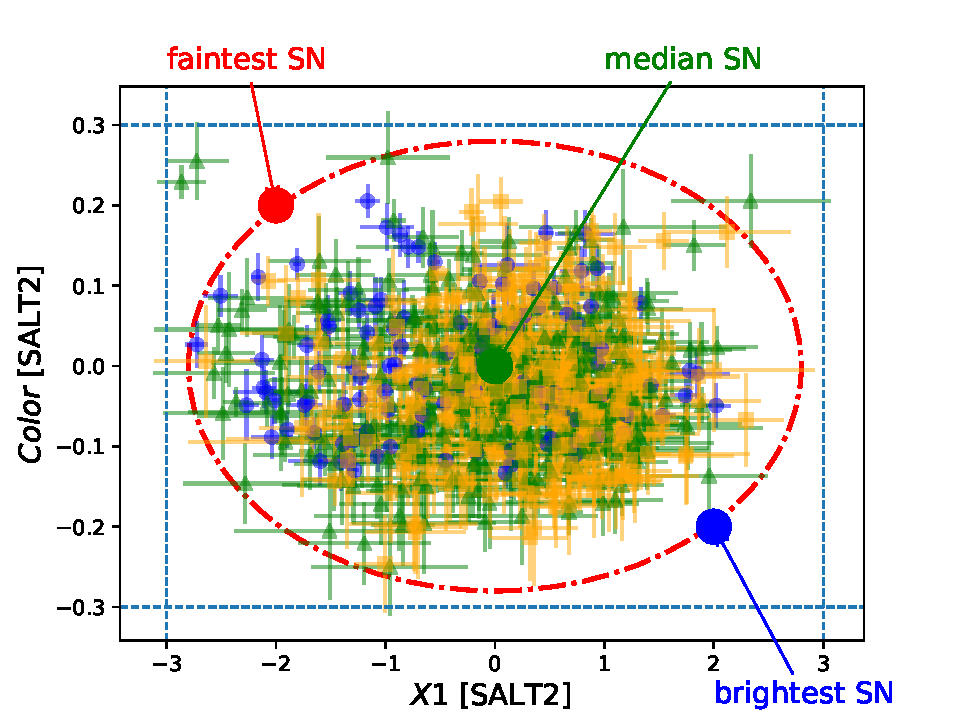
\includegraphics[width=0.6\textwidth]{key_design/sn_parameter_space.pdf}
    \caption{JLA supernovae the $(X_1,Color)$ parameter space --
      (blue: nearby, green: SDSS, orange: SNLS).  The large dots
      indicate the position of the faint, median and bright fiducial
      SNe used for the cadence analyses.}
    \label{fig:jla_X1_C}
  \end{center}
\end{figure}

On the same figure, we have represented three fiducial SNe of
particular interest: the red dot represents the faintest SN in this
region of the parameter space $(X_1=-2, C=0.2)$, the green dot and
blue dots show the average $(X_1=0, C=0)$ and brightest SN $(X_1=2,
C=-0.2)$ respectively.

We can define the redshift limit \zfaint as the limit beyond which the
faintest fiducal SN no longer passes the light curve requirements. By
doing this, we ensure that all SNe that live in the fiducial $(X_1,C)$
parameter space and are below \zfaint do pass our light curve
requirements.  \zfaint defines a {\em redshift-limited sample} whose
selection function does not depend on the SN properties.

We can also define a similar limit, using the median supernova,
instead of the faint one.  This defines a SN sample whose upper
redshift bins are affected by a selection bias, which must be
determined using a simulation -- which itself depends on our knowledge
of the SN luminosity distribution at those redshifts.  The uncertainty
affecting the determination of the selection function generally limits
the usefulness of the redshift bins affected by a selection bias.
Since the selection function is generally symmetric around its 50\%
point, the size of the sample limited by \zmed gives a good
approximation of the total number of LSST SNe that will have precise
distances.

For each cadence we may thus estimate the following quantities in addition to the total number of well-sampled supernovae: 

\begin{itemize}
\item the sample redshift limit, \zfaint defined above, and the number
  of well sampled supernovae below the redshift limit \nsnfaint
\item the redshift \zmed at which the median supernova defined above
  no longer passes the signal-to-noise requirements, and the number of
  well-sampled supernovae below this redshift, \nsnmed.  
\end{itemize}
The former give an assessment of the size and depth of the redshift
limited sample, i.e. the sample of supernovae usable for cosmology,
and whose selection function is extremely easy to determine.  The
latter gives an assessment of the size and depth of the sample of SNe
that will have precise distances.

\subsubsection{Deep Drilling fields}

\myparagraph{Method}

The strategy to estimate the number of well-measured type Ia supernovae may be summarized in four steps: (1) light curves are simulated and fitted using observations of a given cadence; (2) selection criteria are applied to get high-quality supernovae; (3) the resulting observing efficiency curves are then convolved with a production rate \cite{perrett} so as to estimate the number of well-measured type Ia supernovae that may be collected by LSST given an observing strategy. 

Table \ref{tab:sim_ddf} summarizes the parameter used in SN simulations. The selection of a sample of well-measured type Ia supernovae is done in two steps. A sample of observable supernovae is selected by requiring light curves to have \phasemin $\leq$ -5 and \phasemax $\geq$ 20 (where \phasemin~ and \phasemax~ are the minimal and maximum phases of the LC points, respectively). For each supernovae in this reference sample, additional selection criteria are applied:
\begin{itemize}
\item $N_{bef} \geq 4$ and $N_{aft} \geq 10$ where $N_{bef}$ and $N_{aft}$ are the number of LC points (with SNR$\geq$ 5) before and after \daymax.
 \item $\sigma_c \leq 0.04$ where $\sigma_c$ is the error on the \sncolor~parameter estimated from the fit of the light curve.
\end{itemize}
The season length which depends on the redshift is estimated using the supernovae of the reference sample.

\begin{table}[!htbp]
  \begin{center}
    \caption{Range of the parameters used to simulate type Ia SN}\label{tab:sim_ddf}
\begin{tabular}{cc}
  \hline
  \hline
Parameter & Range \\
\hline
\hline
                    & (-2.0,0.2),(0.0,0.0),(2.0,-0.2) \\
 (\strech,\sncolor) & (-2.0,0.0),(-2.0,0.2),(0.0,-0.2) \\
                    & (0.0,0.2),(2.0,0.0),(2.0,0.2) \\
\hline
\redshift           & [0.01,1.3] (step: 0.025) \\
\hline
\daymax             & [\tmin,\tmax] (step: 1 day) \\
                    & (\tmin~and \tmax~ are the min and max MJD of a season) \\
                    \hline
\end{tabular}
\end{center}
\end{table}

\myparagraph{Results}

Typical detection efficiencies are given on Fig. \ref{fig:effi} for the \cosmos~field and feature\_baseline\_10 yrs cadence . One may observe that the lowest efficiencies (independently on the (\strech,\sncolor) values) correspond to the first two seasons of observations which are known to be very bad for this observing strategy and for this field (see for instance Figs. \ref{fig:cosmoscad} and \ref{fig:cosmos_m5}).

\begin{figure}[htbp]
\begin{center}
  
  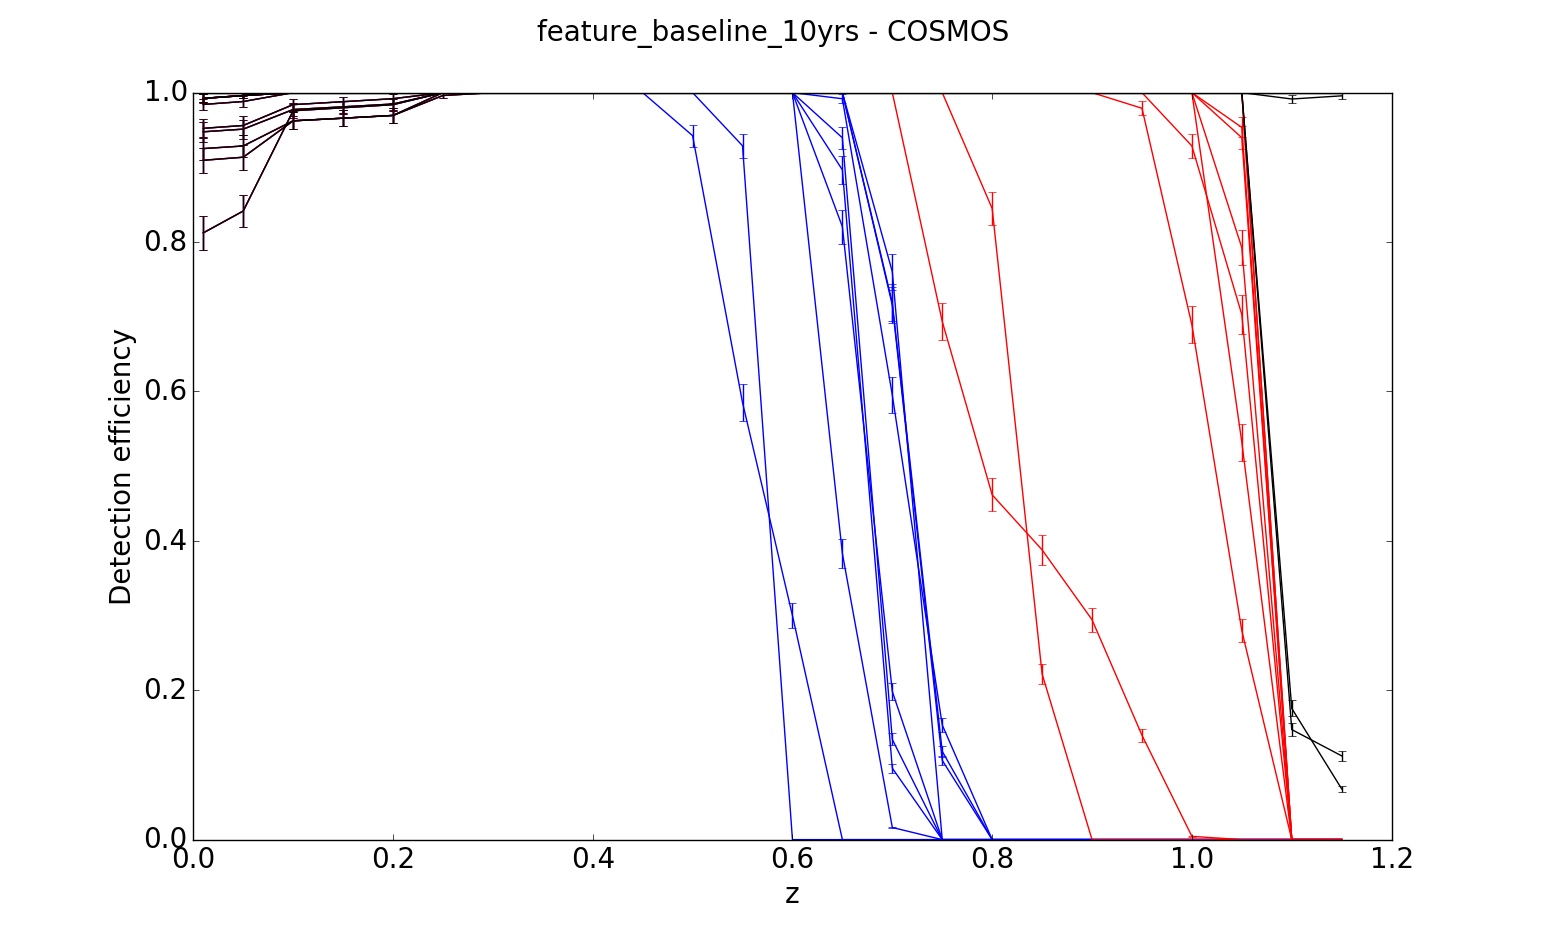
\includegraphics[width=12cm]{nsn/effi_feature_cosmos.png}
 \caption{Detection efficiency as a function of the redshift for the \cosmos~field and feature\_baseline\_10yrs observing strategy (10 seasons). Blue, red and black lines correspond to faint, medium and bright supernovae, respectively.}\label{fig:effi}
\end{center}
\end{figure}

Efficiency curves are convolved with a production rate \cite{perrett} to estimate the number of well-measured type Ia supernovae that may be collected by LSST. Summary plots are given for the reference fields (Fig \ref{fig:nsn_four}) and for all the DDF (Fig \ref{fig:nsn_all}). One may observe that, despite bad observing years, \feature~ shows the best results in terms of number of well-measured type Ia supernovae. Equivalent results are obtained with Colossus\_2667.

\begin{figure}[htbp]
\begin{center}
  
  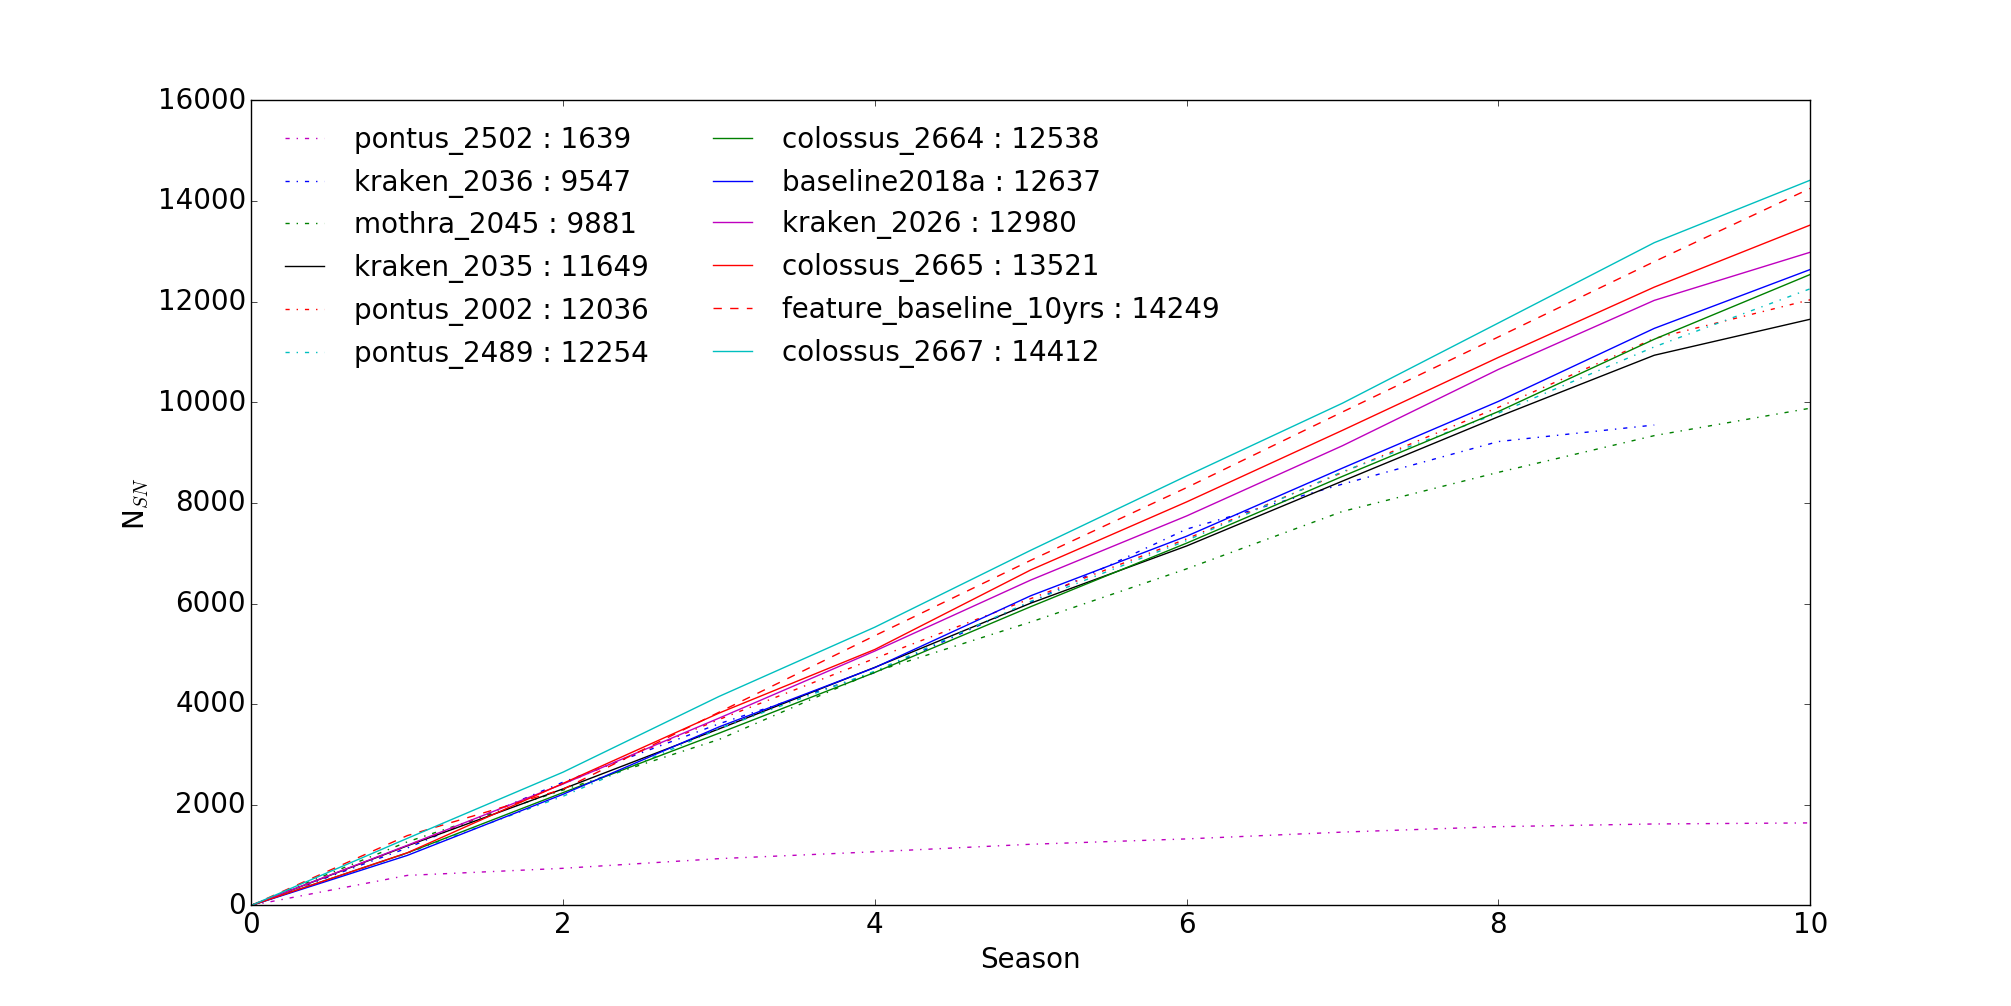
\includegraphics[width=15cm,height=10cm]{nsn/NSN_season_4DDF.png}
  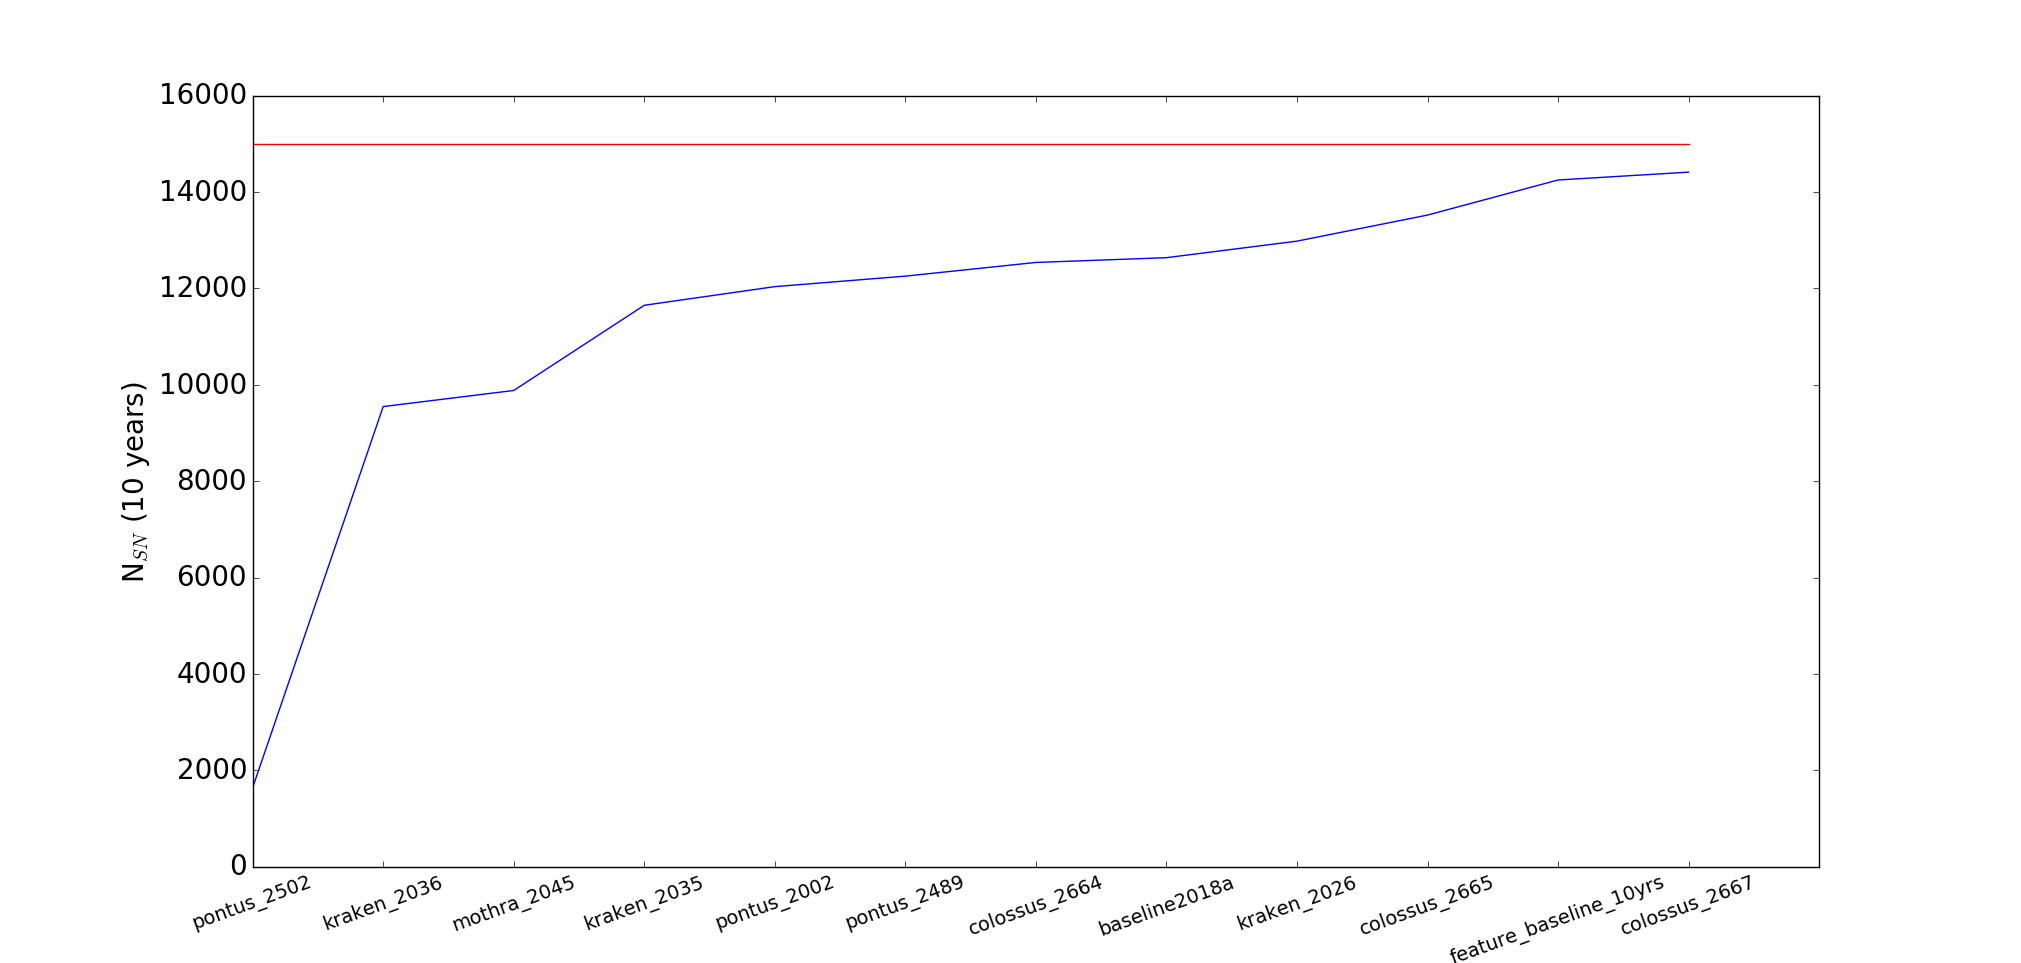
\includegraphics[width=15cm,height=10cm]{nsn/NSN_all_4DDF.png}
 \caption{Top: Number of well-measured type Ia supernovae as a function of the season. Bottom: Number of  well-measured type Ia supernovae as a function of observing strategy after ten years of operation. Four DDF (\cosmos,\xmmlss,\cdfs,\elais) have been considered.}\label{fig:nsn_four}
\end{center}
\end{figure}

\begin{figure}[htbp]
\begin{center}
  
  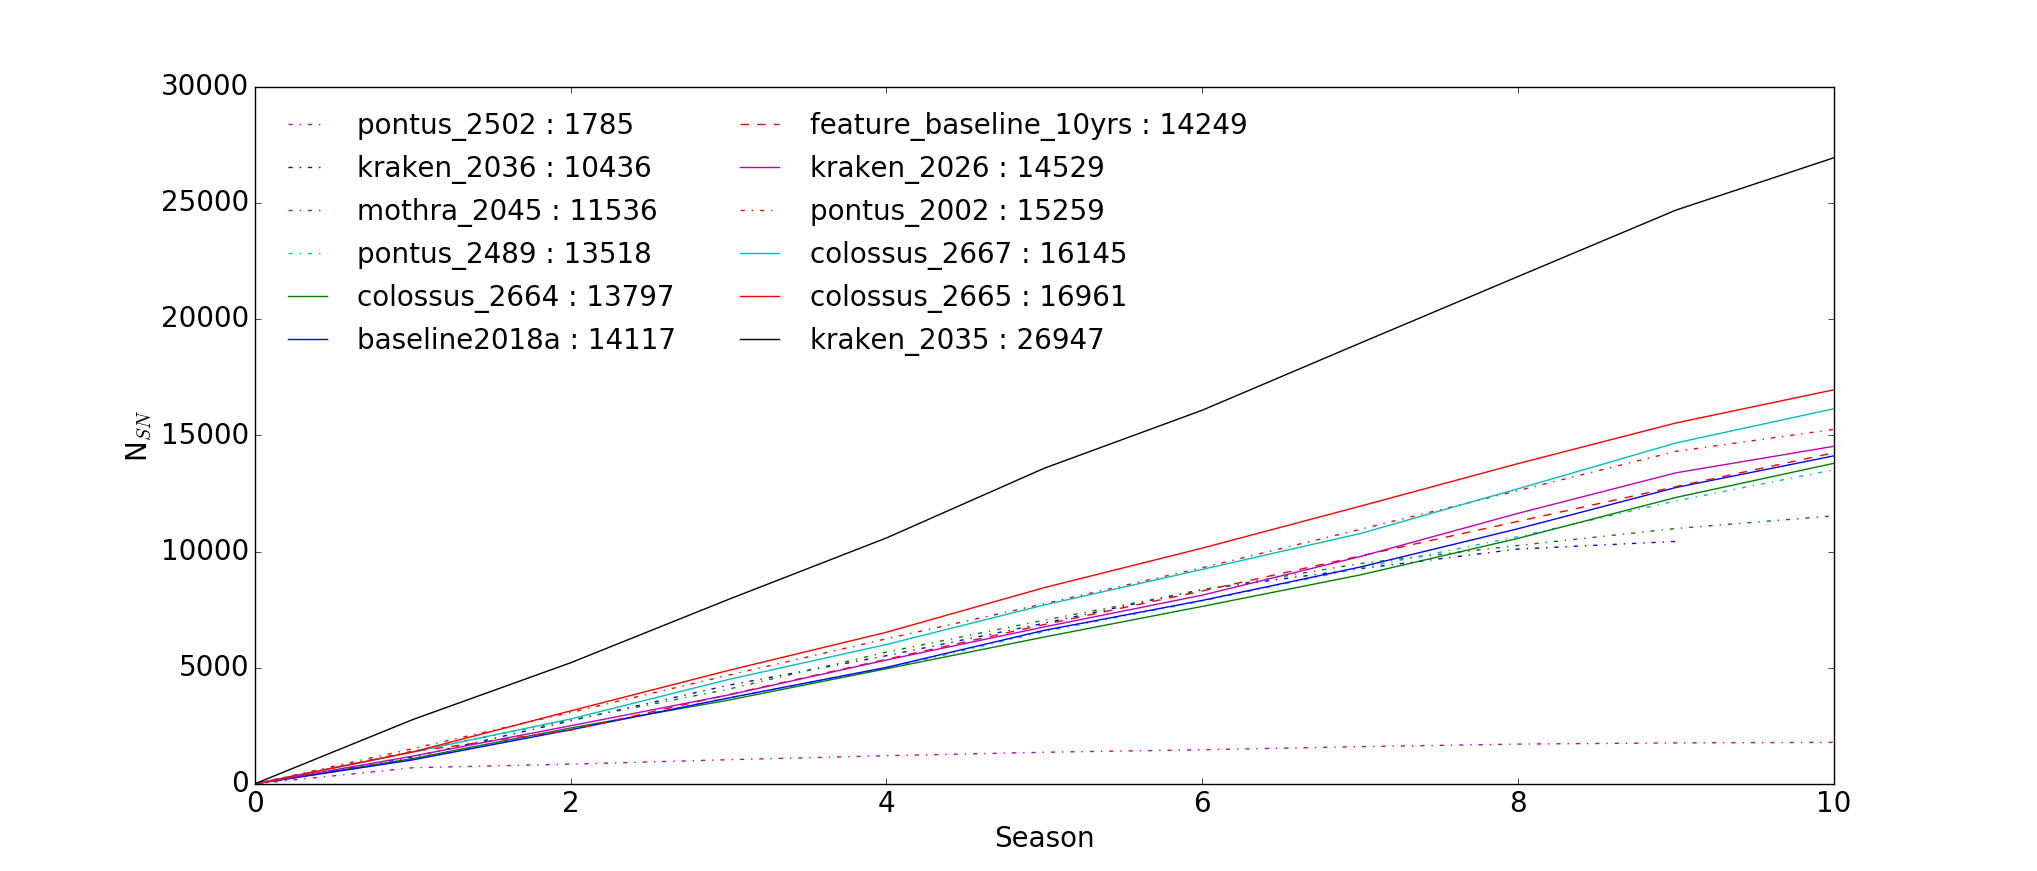
\includegraphics[width=15cm,height=10cm]{nsn/NSN_season_allDDF.png}
  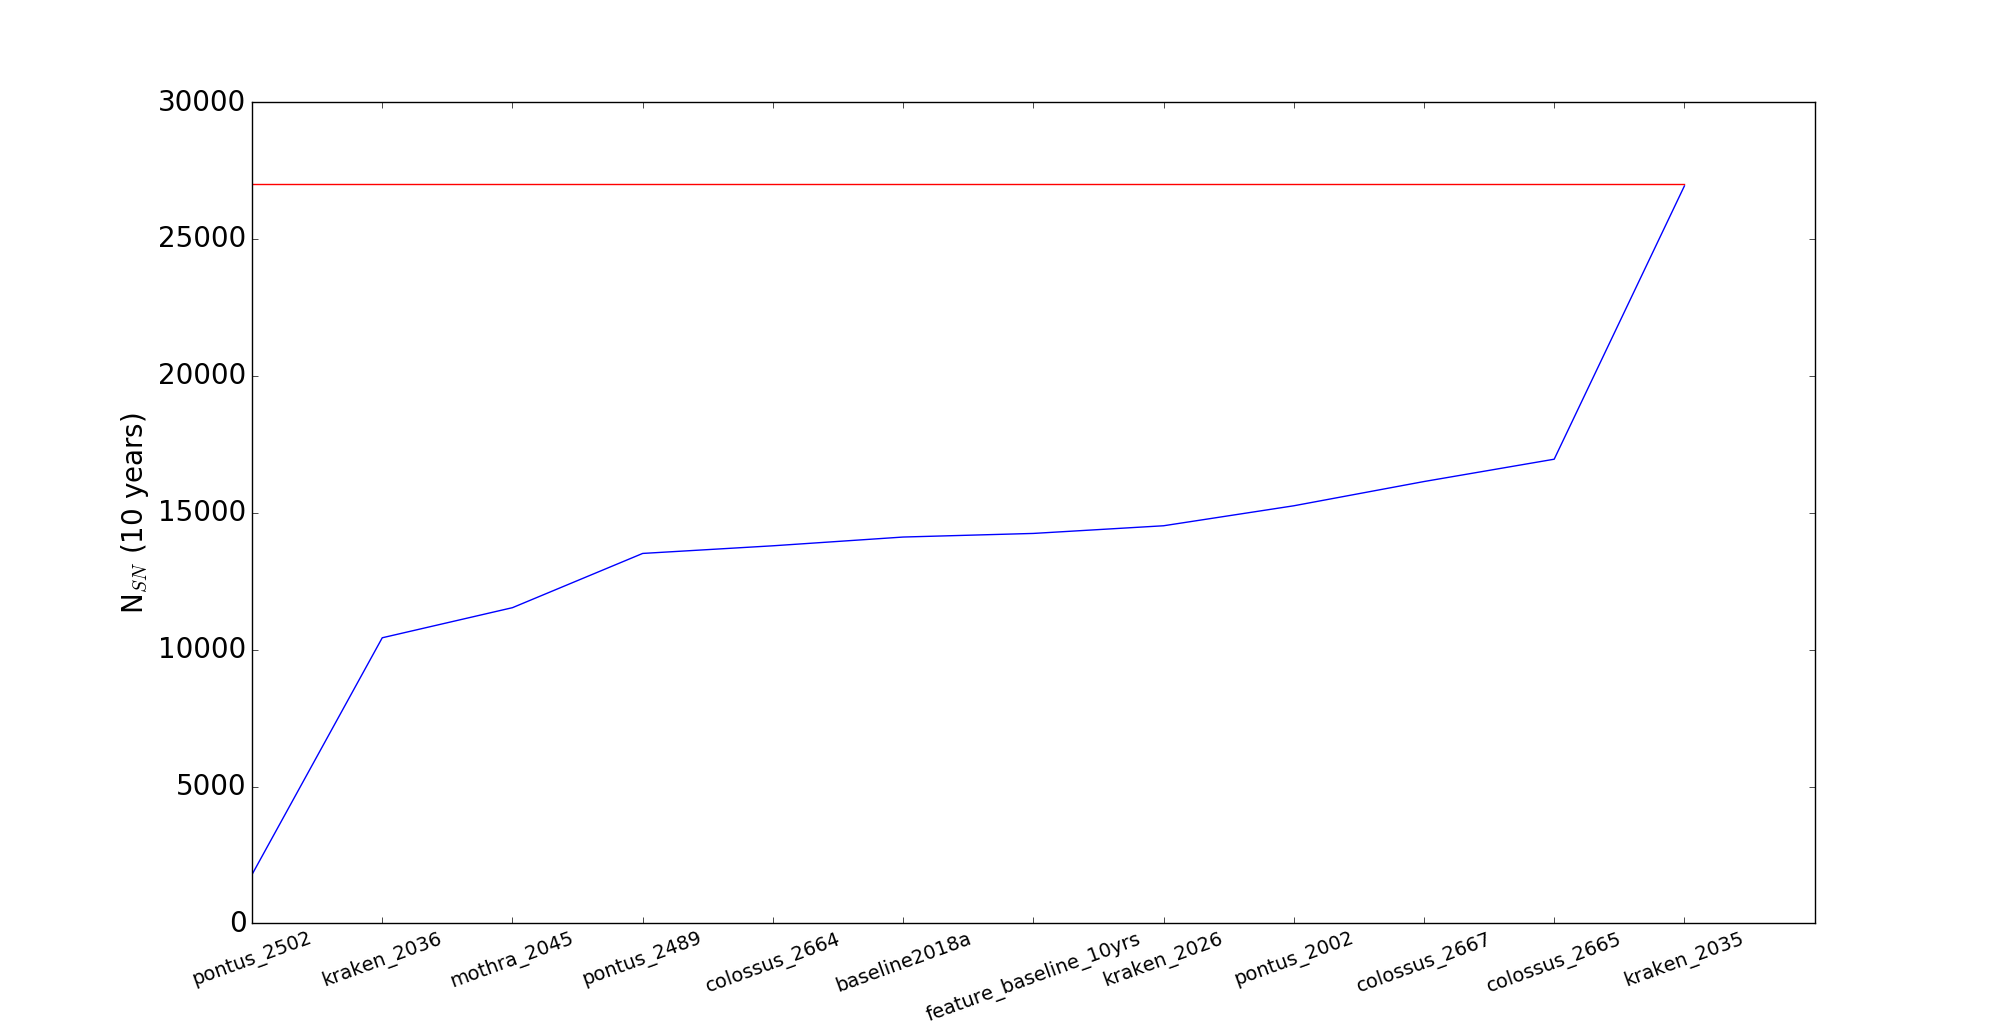
\includegraphics[width=15cm,height=10cm]{nsn/NSN_all_allDDF.png}
 \caption{Top: Number of well-measured type Ia supernovae as a function of the season. Bottom: Number of  well-measured type Ia supernovae as a function of observing strategy after ten years of operation. All DDF have been considered.}\label{fig:nsn_all}
\end{center}
\end{figure}

\myparagraph{Conclusion}

When considering all DDF the winner (w.r.t. the total number of well-sampled supernovae) is of course kraken\_2035 (30K after ten years) since this observing strategy considered 9 DDFs whereas all others observed 4 to 5 fields. One may observe that extrapolating a four fields configuration results (like the ones obtained with \feature) to a 9 DDF observing strategy will probably lead to an overestimation of the resulting number of well-measured type Ia supernovae. It is indeed difficult to maintain the same quality (in terms of cadence, season length and thus depth) when moving from a 4 to a 9 DDF strategy.

\begin{sidewaysfigure}
\begin{center}  
  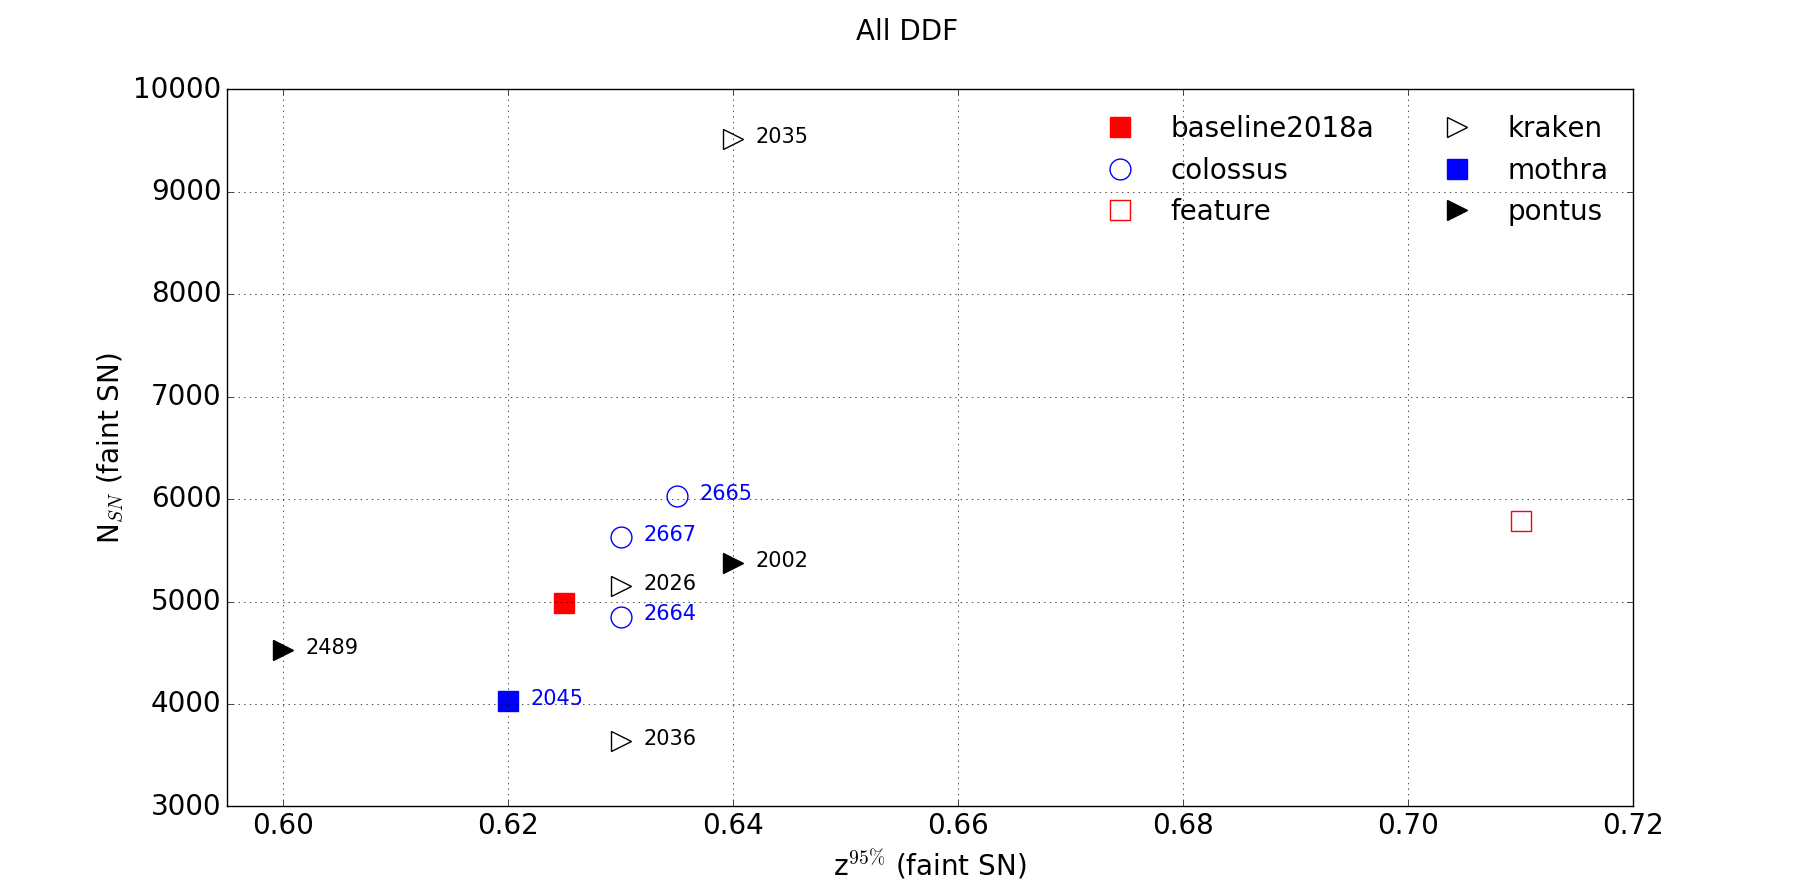
\includegraphics[width=\linewidth]{nsn/Z95_NSN.png}
 \caption{Median 95\% redshift limit (ie corresponding to the detection of 95\% of the faint supernovae sample) as a function of the number of supernovae (with $z\leq z_{0.95}^{faint}$).}\label{fig:z95}
\end{center}
\end{sidewaysfigure}

\begin{sidewaysfigure}
\begin{center}  
  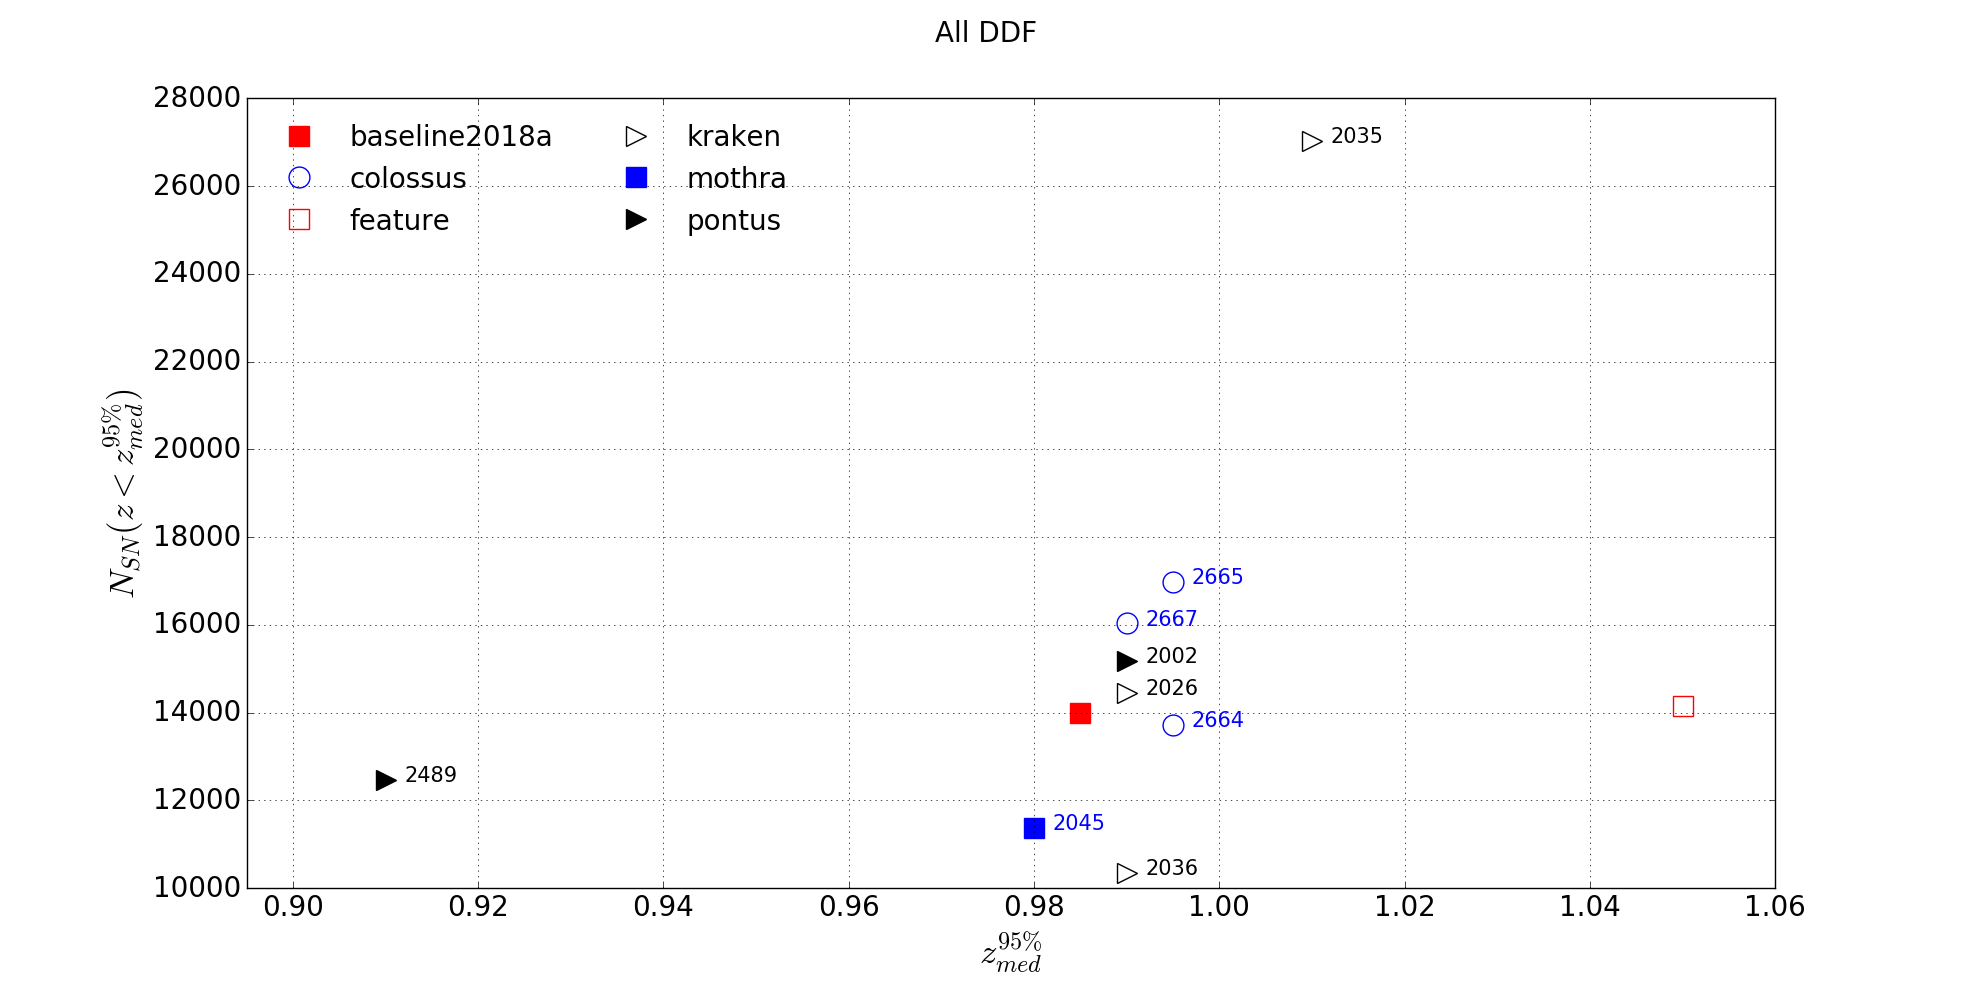
\includegraphics[width=\linewidth]{nsn/Z95_NSN_med.png}
  \caption{Median 95\% redshift limit (ie corresponding to the detection of 95\% of the medium supernovae sample) as a function of the number of supernovae (with $z\leq z_{0.95}^{med}$).}\label{fig:z95_med}
\end{center}
\end{sidewaysfigure}



Another way to assess the quality of an observing strategy is to estimate the redshift detection limit for faint or medium supernovae (see \ref{sec:metrics}). On Figures \ref{fig:z95} and \ref{fig:z95_med} are  displayed the 95\% redshift limit (ie corresponding to the detection of 95\% of the faint or medium supernovae sample) as a function of the number of supernovae (with  $z\leq z_{0.95}$). Huge variations among and inside strategies are observed. This plot reflects the quality of the proposed cadences. It seems that \redshift~of 0.7-0.75 may be reached with four fields. Once again \feature~tend to give the highest redshifts and the most homogeneous results among the fields and seasons. 


\subsubsection{Wide Fast Deep}
\label{sec:wide_fast_deep_analysis_method}

\myparagraph{Method}

WFD observations involve a large number of fields.  The observations
are dithered, and the size and depth of the final sample depends
heavily on the details of the observing strategy (in particular, the
filter allocation strategy and the field selection function \ldots)
For this reason, we opted for a slightly different approach, which we
describe below.

The celestial sphere is pixellized in Healpix superpixels\footnote{we
  choose nside=64, which corresponds to 0.8 deg$^2$ healpixels.  We
  have verified that (1) larger pixels (nside=32) leads to
  underestimating the number of SNe by \~ 15\% and
  that smaller pixels (nside=128 and above) give exactly the same
  results.}.  The directions / healpixel affected by a Galactic extinction $E(B-V)$ larger than 0.25
are masked and not included in our assessment. We consider only the $griz$ observations which are the ones
that matter to derive SN luminosity distances. 
Using a simple model of the LSST focal plane, we play
the cadence, and estimate the list of superpixels observed for a
given exposure. This allows us to build a log which reports the mjd,
band, and observing conditions of each healpixel observation.

We can then analyze this log, using as a probe, a fiducial SN~Ia,
e.g. the ``faint'' or ``normal'' SNe~Ia defined in the previous
section. For each mjd and each pixel, we determine:
\begin{eqnarray}
  z_{\mathrm{lim}} & = & \mathrm{max}\left(z | \mathrm{LC(z)\ fulfill\ requirements}\right) \\
  N_{z<z_{\mathrm{lim}}} &= & \delta\Omega_{\mathrm{pix}} \int_0^{z_\mathrm{lim}} \frac{\Delta T_{\mathrm{step}}}{1+z}\ {\mathcal{R}}(z)\ dV(z)
\end{eqnarray}
where $\delta\Omega_{\mathrm{pix}}$ is the solid angle subtended by
one pixel, $\Delta T_{\mathrm{step}}$ is the simulation time step (in
observer frame days) and $\mathcal{R}(z)$ is the SN~Ia volumetric rate
(we adopt the rate published in \cite{perrett}).  We also
compute the average cadence (in day$^{-1}$), i.e. the number of $g, r,
i$ or $z$ visits in a fiducial restframe interval.

The quantities above are determined for each pixel and each night
(identified by its mjd).  We report them in full sky maps, which give
an assessment of how the cadence performs in a $\sim 50$ day time
interval around the current mjd. From these maps, we can build global
maps giving, as a function of the position on the sky (1) the density
of supernovae (2) the median maximum redshift (3) the median cadence.
We can also collate these maps in videos, that are useful to evaluate
the observing strategy as a function of time.

\begin{sidewaysfigure}
    \begin{center}
      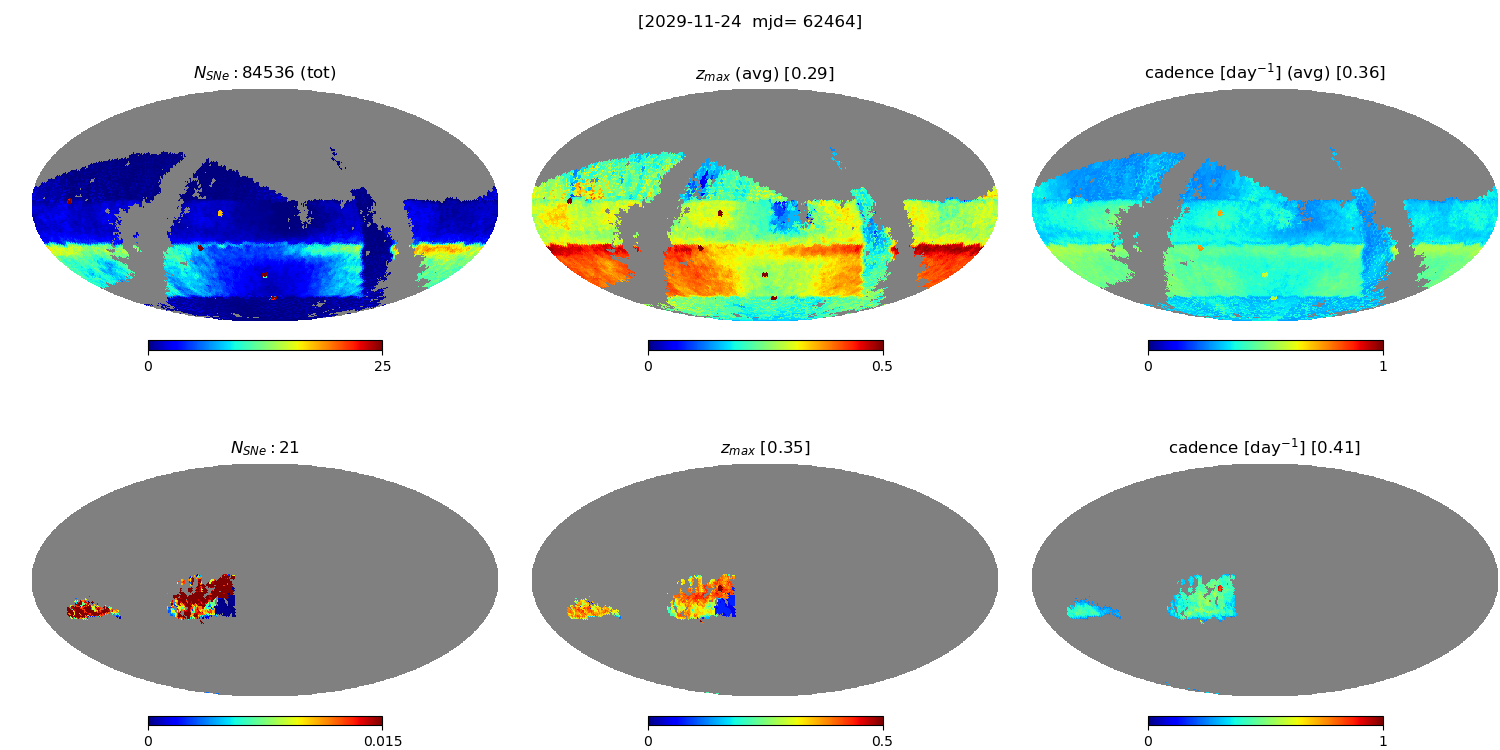
\includegraphics[width=\linewidth]{nsn/mothra_2045_02611.png}
      \caption{Example of cadence analysis maps.  Cadence {\em
          Mothra\_2045}, mjd=62464 (2029-11-24) {\em Upper panels:}
        (left) total number of well sampled supernovae per healpixel,
        (middle): median \zmed after 2611 days of survey, (right):
        median cadence, after 2611 days of survey. {\em Lower panels:}
        (left) number of SNe~Ia peaking at mjd=62464 and passing the
        light curve quality cuts (middle) \zmed, i.e.  maximum
        redshift at which a SN peaking at mjd=62464 would pass the
        requirements}
    \end{center}
\end{sidewaysfigure}

\myparagraph{Results}

We have conducted the analysis described above on all the cadences released
so far.  The final maps that report, for each healpixel (1) the final
number of SNe (2) the mean redshift limit
($\left<z_{\mathrm{faint|med}}\right>$) reached (3) the average
(restframe) cadence obtained are included in appendix
\ref{sec:wfd_maps} (figures \ref{fig:altsched_rolling_good_weather} to
\ref{fig:feature_baseline}). Finally, the animations that show the evolution
of the maps as the survey unfolds are available at the following address:
\begin{center}
  \href{http://supernovae.in2p3.fr/~nrl/lsst_sn_cadence}{http://supernovae.in2p3.fr/\~{}nrl/lsst\_sn\_cadence}
\end{center}
Inspecting these maps, we essentially recover the ranking of cadences
presented in the previous section.  We note that on some cadences,
especially the rolling cadences, the average properties (size and
depth) of the SN sample vary significantly as a function of the sky
direction. Some of these effects are related to seasonality (better
seeing allows to go deeper, for example) and depend on how realistic
the \opsim weather and seeing logs are. Others are clearly artefacts
of the observing cadence and can be corrected. For example, the on the
{\tt Mothra} and {\tt SLAIR} rolling cadences, are lines clearly
visible which correspond to depleted regions at the boundary between
the areas observed each year. The same is true on altsched rolling,
which also displays a strongly depleted region, at the region where
the scheduler switches between the upper and lower declination area.
Cures exists for these effects and are being discussed. 

Our primary metrics, ($z_{\mathrm{faint|median}}$, $N_{\mathrm{faint|median}}$) 
presented in section \ref{sec:metrics}, can be derived from these
maps.  Figures \ref{fig:nsn_zmax_med} and \ref{fig:nsn_zmax_faint}
give a synthetic presentation of our cadence evaluation, in the planes
(\zfaint, \nsnfaint) and (\zmed, \nsnmed), respectively.

\begin{sidewaysfigure}
  \begin{center}
    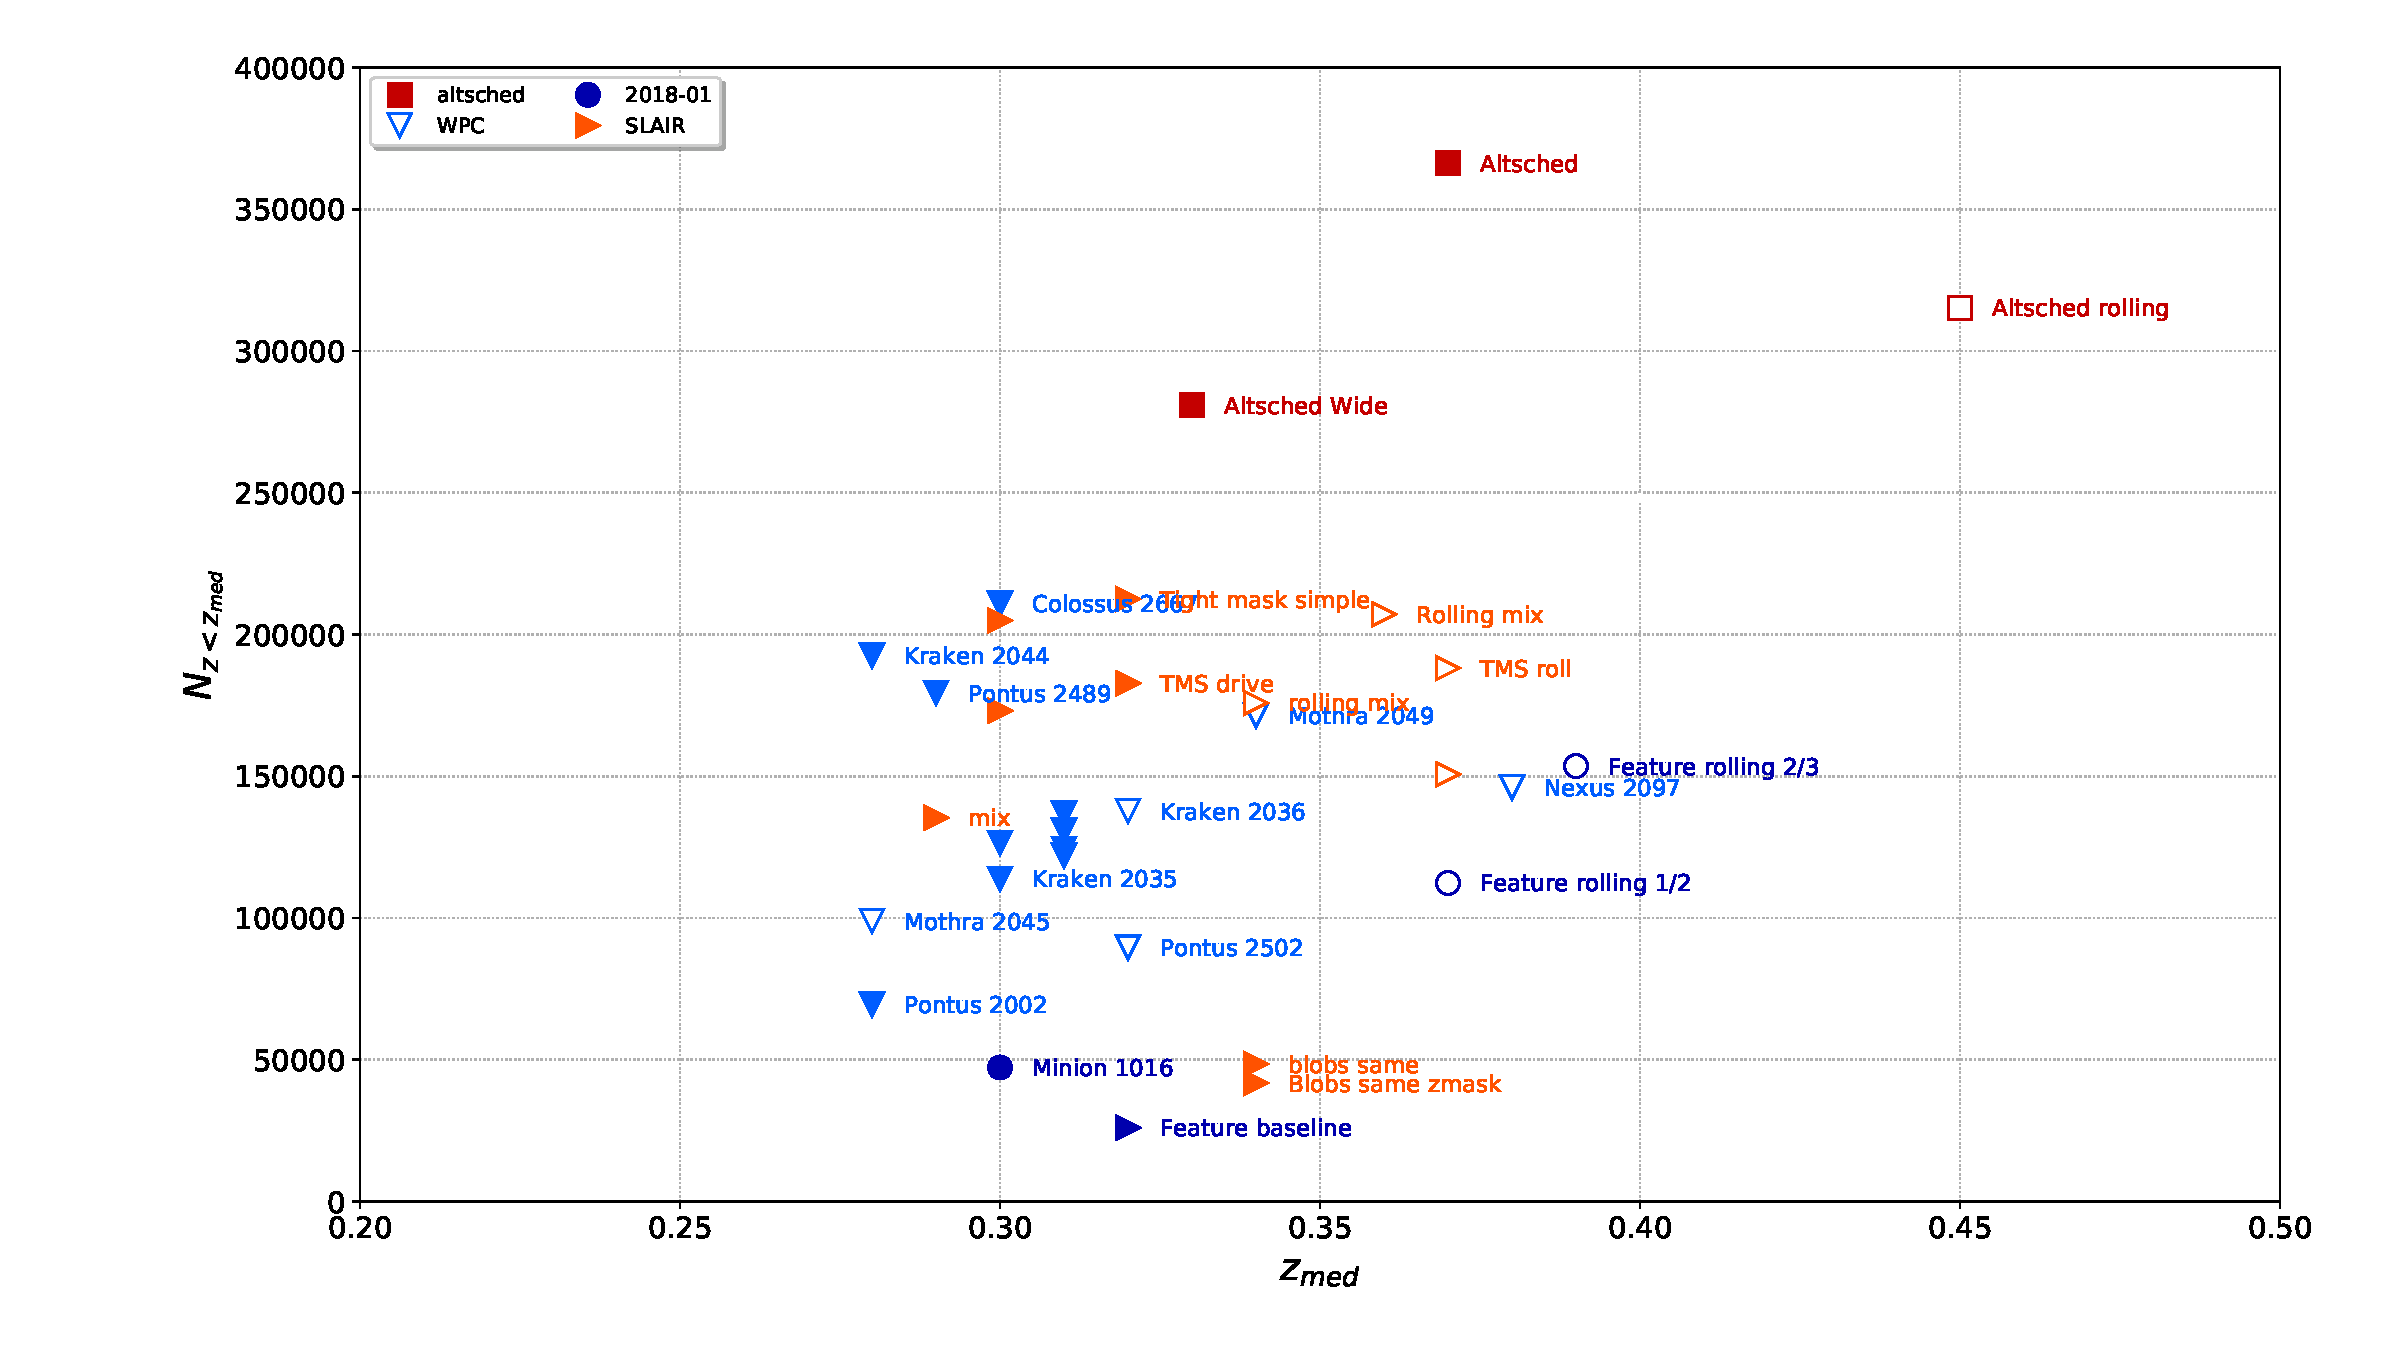
\includegraphics[width=\linewidth]{nsn/summary_plot_wfd_mediansn.pdf}
    \caption{Representation of the cadences analyzed in this study in
      the plane (\zmed, \nsnmed). This gives an assessement, for each
      cadence, of (1) the sample depth, i.e. at which redshift the
      median SN no longer passes the requirements listed in section
      \ref{sec:sn_sampling_requirements} and (2) the size of the
      subset of well-sampled SNe~Ia.}
    \label{fig:nsn_zmax_med}
  \end{center}
\end{sidewaysfigure}

\begin{sidewaysfigure}
  \begin{center}
    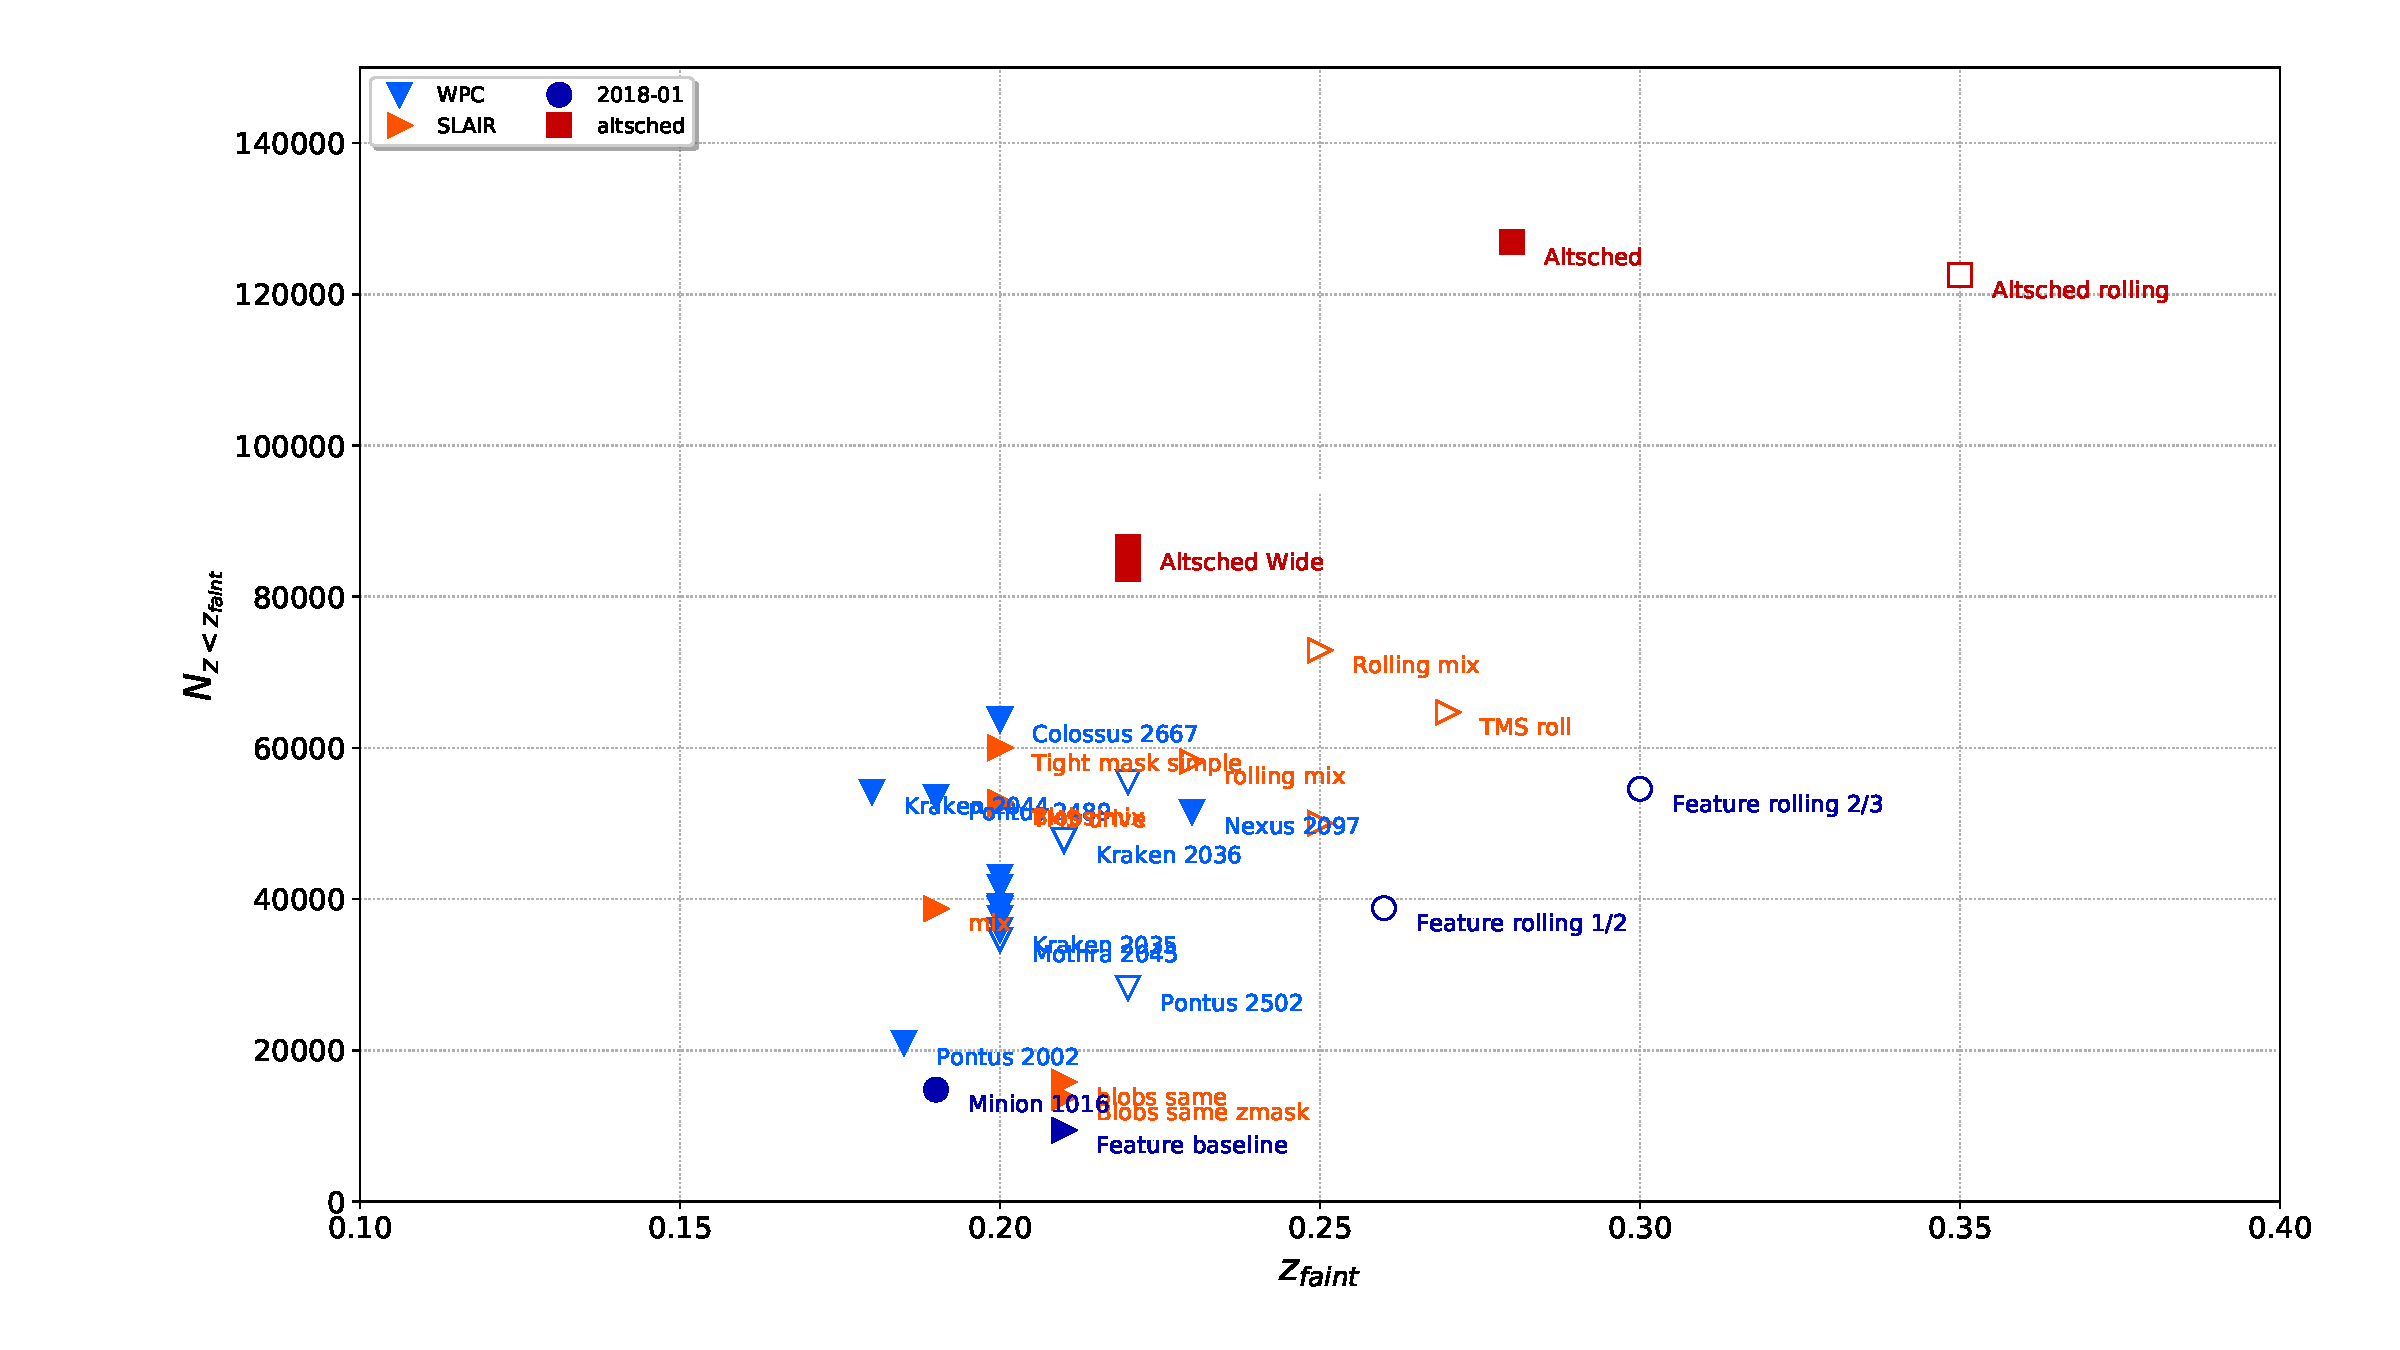
\includegraphics[width=\linewidth]{nsn/summary_plot_wfd_faintsn.pdf}
    \caption{Representation of the cadences analyzed in this study in
      the plane (\zfaint, \nsnfaint). This gives an assessement, for
      each cadence, of (1) the redshift limit of the survey, i.e. at
      which redshift the faintest SN no longer passes the requirements
      listed in section \ref{sec:sn_sampling_requirements} and (2) the
      size of the redshift limited SN~Ia sample produced by LSST.}
    \label{fig:nsn_zmax_faint}
  \end{center}
\end{sidewaysfigure}

Again, we recover our previous ranking.  The rolling version of
\altsched is the best performing cadence.  It will allow us to build a
very deep sample \zmed $\sim 0.45$ of more than well sampled 300,000
SNe.  {\tt altsched} covers more area, at the expense of a lower
cadence.  As a consequence, it is not as deep, but allows to obtain a
larger number of well-sampled SNe.

Most of the cadences released for the white paper call do not allow to
go as deep, no to secure as many well sampled SNe. The best \opsim and
\slair rolling cadences allow to reach redshift limits that are
similar to the non-rolling version of \altsched and yield samples that
are about 40\% smaller. All of them, in particular {\tt rolling mix}
and {\tt tms roll} implement the design principles exposed in section
\ref{sec:wfd_cadence_key_properties}. Why they do not reach the
performances of {\tt altsched rolling} is unclear at this point and is
being investigated.
